\chapter{Shark Engine}
\label{sec:sharkengine}

\section{Architectur}
Figure \ref{fig:sharkComponents} illustrates the major components which are discussed in a little more detail in this section.

\begin{figure}[t]
\centering
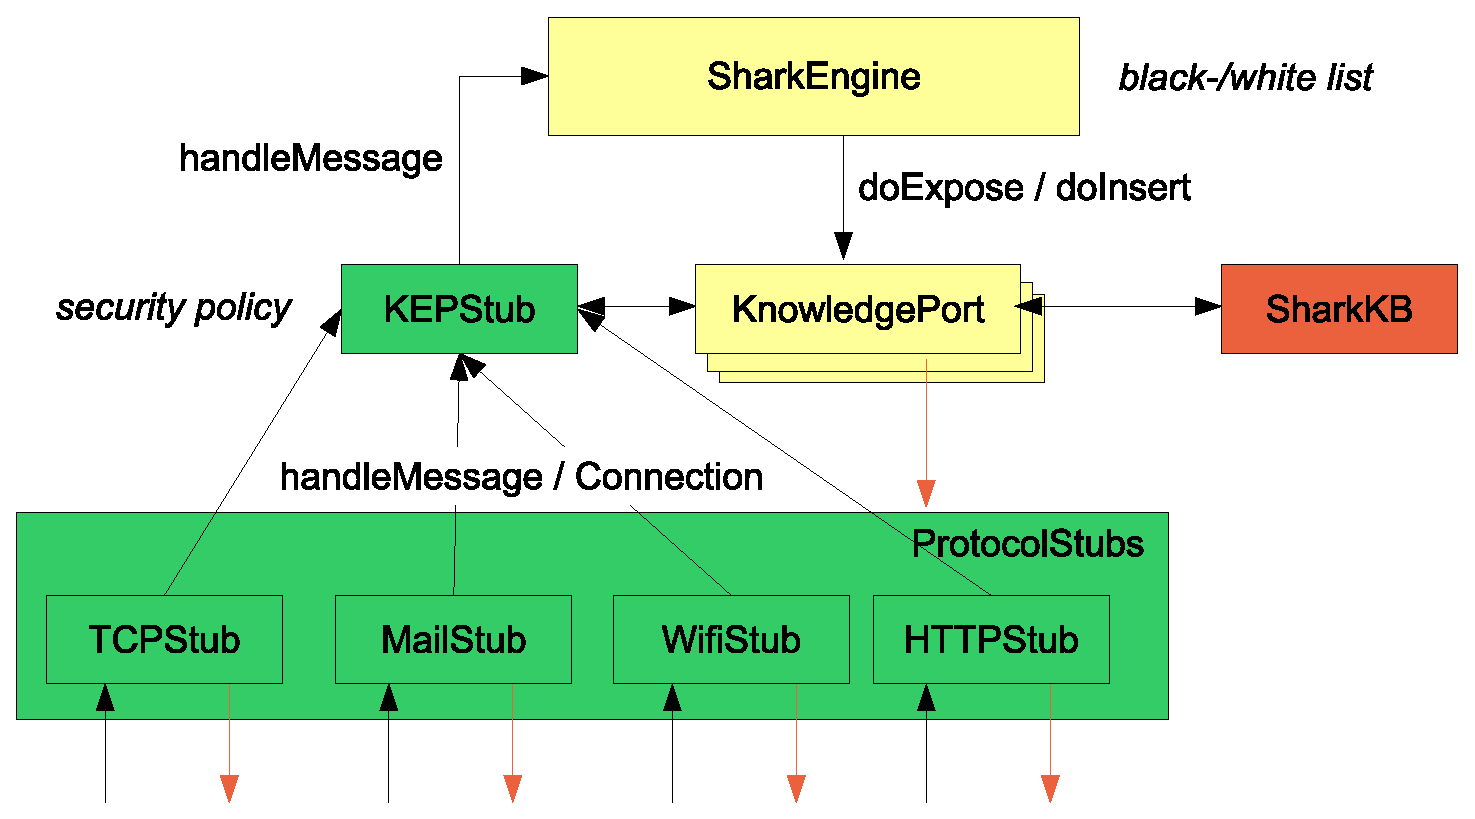
\includegraphics[width=1.00\textwidth]{sharkComponents.eps}
\caption{Shark components}
\label{fig:sharkComponents}
\end{figure}

\subsection{Stubs}
Let's start with the {\it protocol stubs}. Shark supports TCP and E-Mail in version 2. HTTP will be supported soon\footnote{which is quite simple because HTTP is actually a TCP stub with an additional HTTP header} and Wifi-Direct which is already working in the laboratory but requires further tests to be officially added to the system.

Each stub is actually protocol server and client. The TCP stub supports e.g. a method to send data to another peer via TCP. The same stub comprises a TCP server as well which accepts new connections. Developers won't get bothered with those details anyway.

Server parts of each stub just receives messages (e.g. with POP3) or establish connection (TCP and Wifi). Management of this data and connections is handled by the {\it KEP Stub}.

The {\it KEP stub} takes data from underlying protocols and tries to parse a KEP message. It decrypts messages and verifies signatures if required and checks if message comply with defined security policies (which are explained in chapter \ref{sec:security}). Parsing and security methods can fail. {\it KEP stub} writes a log messages and throws any data away. Valid KEP messages are given to the {\it SharkEngine}. 

\subsection{SharkEngine}
The engine has a very little job in KEP message handling. Developers can maintain black- and white lists in the engine. Only KEP messages from allowed senders are accepted. All others are simply dropped without further actions.

The engine also keeps a list of active knowledge ports. The engine checks whether the KEP message contains an {\it interest} or {\it knowledge} and calls {\tt doExpose} or {\tt doInsert} on each active knowledge port.

\subsection{Knowledge Port}
We have already discussed knowledge ports and their usage. The can work with a local knowledge base. Knowledge ports can reply to the sender. In most cases, an already established connection is used. Knowledge ports can also decide to send messages to other addresses. In this case, the KEP stub is used to create a new connection. Developers are not aware of using KEP stub or protocol stubs. They just use the {\tt KEPConnection} interface.

\subsection{Message2StreamStub}
{\it Interest} are usually small in terms of number of bytes. {\it Knowledge} can be huge. Huge data is no problem in general when using a stream protocol like TCP. It becomes a problem when using message oriented protocols like e-mail. 

We had serious discussions how to deal with that problem. An e-mail has a limited length. It depends on capacity and policy of recipient's mail server. What can be done if a KEP message exceeds that limit? In general, there are two possible way:

\begin{enumerate}
    \item Throwing an exception. That would make the framework easier to implement. Unfortunately, developers would be responsible to ensure that KEP message has a maximum size.
\item The framework solves that problem. 
\end{enumerate}

We have chosen the second option. Developers can ignore length of KEP message or send knowledge. There is the {\tt Message2StreamStub} class inside the framework. It takes a message based protocol like SMTP and makes it usable as a stream protocol. It makes a little flow control. The principle is simple: KEP messages which exceed the maximum message length are split into $n$ messages. Each message gets its own number beginning with 0 and the maximum number. Recipients acknowledge received messages which triggers the next package. Developers don't have to care about this little flow control. The behavior can be visited by observing mailboxes used by peers.

In any case, large data are only transmitted via e-mail if no other protocol is available. Its throughput is awful. We come back to that point in section \ref{sec:se:protocolPriorities}

\section{Knowledge Port Management}
Knowledge ports are managed by the Shark engine. Developers don't have to add a knowledge port to the engine. It is done by the {\tt KnowledgePort} constructor.

Each constructor requires at least a Shark engine as parameter. There was e.g. this line in our Alice program:

\begin{verbatim}
SharkEngine aliceSE = ...;
StandardKP kp = new StandardKP(aliceSE, cc, aliceKB);
\end{verbatim}   

The constructor adds the port to the engine. Knowledge ports can be deleted:

\begin{verbatim}
aliceSE.deleteKP(kp);
\end{verbatim}

Object {\tt kp} is removed from the list of knowledge ports. It cannot be added. The only way is to create a new knowledge port with same parameters. Knowledge ports can be activated and deactivated. That's a feature of knowledge ports, see section \ref{sec:knowledgePorts}.

All knowledge ports can be retrieved.
\begin{verbatim}
aliceSE.getAllKP();
\end{verbatim}

\subsection{Publishing}
Each engine offers methods to start or re-start a conversion between peers.
Let's have a look at the following code.

\begin{verbatim}
PeerSemanticTag remotePeer = ...;
aliceSE.publishKP(kp, remotePeer);
\end{verbatim}

Engine takes the interest which is stored in the knowledge port. This interest is sent as {\it KEP expose} to {\tt remotePeer}.

\begin{verbatim}
aliceSE.publishKP(kp);
\end{verbatim}

This method is similar to the previous version. Recipients are extracted from {\tt kp} interest: Each peer {\it remote peer dimension} gets an expose message.
Apparently, it only works if this dimension is not empty.

\begin{verbatim}
aliceSE.publishAllKP(remotePeer);
\end{verbatim}

This method publishes any knowledge port to {\tt remote peer}.

\begin{verbatim}
aliceSE.publishAllKP();
\end{verbatim}

This method iterates over all knowledge ports and performs an {\tt publishKP(kp)} on each of them.

\section{KEP communication}
\label{ref:sec:KEP}
We have already seen that {\tt KEPStub} orchestrates communication and hides protocol specifics and security algorithms from developers. {\tt KEPStub} provides several other, maybe, useful methods which are discussed in this chapter. 

Developer don't have to access {\tt KEPStub} directly. Shark engine acts as {\it facade}: It offers methods and delegates parts of their duties to other components. Thus, sometime we might intermix {\tt KEPStub} and {\tt SharkEngine} in the next section. Don't care: Any method is available on the {\tt SharkEngine} interface. Internals are of no interest for Shark application developers.

\subsection{Communication History}
Peers send and receive messages. Received message can be handled by knowledge ports or not. The later are called {\it unhandled messages}. Sending can fail. Shark is meant to be a framework for spontaneous networks. Communication breakdown must be seen as usual event and not as avoidable error. Messages that are ought to be sent are stored and can be re-sent later.

The following methods are offered by {\tt SharkEngine}.

\begin{verbatim}
// returns all interests exposed since a given point in time
Iterator<SharkCS> getSentInterests(long since);

// returns all knowledge sent since a given point in time
Iterator<Knowledge> getSentKnowledge(long since)
  
// returns interests which are not handled by any knowledge port
Iterator<SharkCS> getUnhandledInterests(long since)

// returns background knowledge of knowledge that wasn't handled by
// any knowledge prt
Iterator<SharkCS> getUnhandledKnowledge(long since);
\end{verbatim}

First three methods are obvious. {\tt getUnhandledKnowledge} returns a context space but no knowledge. That's because of resource considerations. Knowledge tends to be huge. Context spaces are quite small compared to knowledge. Knowledge arrives with {\it KEP insert}. Active knowledge ports have the chance to assimilate that knowledge. The engine stores the background knowledge of non-assimilated knowledge but not knowledge itself. Background knowledge contains any necessary information to get that knowledge again. Thus, applications could iterate non-assimilated background knowledge and issue {\it KEP expose} requests to the other peers which can re-sent that knowledge.

\subsection{Silent period and empty knowledge}
{\tt KEPStub} keeps track of sent interests and knowledge. It checks whether 
or not those messages were already sent and sometimes prevents the system from sending. 
It is a very useful feature especially for spontaneous networks which tend to stutter. Let's explain it by an example:

We are familiar with the Alice and Bob basic communication scenario. Imagine that applications runs on mobile phones which communicate solely with Wifi-direct. Alice and Bob e.g. meet at a table having lunch. Their devices establish a connection. At least one device issues an interest after a connection establishment. The communication takes place - anything it fine.
Imagine, Bob stands up e.g. to go for some tomato sauce. Wifi communication breaks down more or less immediately. It is re-established when he comes back.
Thus, one peer would issue the same interest as minutes before, both devices would perform same communication again and again. That additional power consumption would be a heavy burden for mobiles phones accumulator.

There is a {\it silent period}. {\tt KEPStub} don't issues identical KEP messages within that silent period. Identical means identical content and identical recipient. When Bob returns, one device might prepare for sending the same interest again but {\tt KEPStub} would prevent from sending that message.

That period can be set.
\begin{verbatim}
public void setSilentPeriod(int milliseconds);
\end{verbatim}

There is a default setting defined in {\tt DEFAULT\_SILTENT\_PERIOD}.

Nevertheless, it is useful to re-expose interests to other peers. That's what we do when we read or listen to our preferred news paper / channel. Maybe the other peer has new information.

{\tt KEPStub} keeps track of delivered knowledge. Identical knowledge won't be sent again. {\tt KEPStub} uses a history for that reason which can be removed.

\begin{verbatim}
// removes expose and insert history
removeSentHistory();
\end{verbatim}
Afterwards, the system has forgotten its history and would send any knowledge.

There is a final quite special scenario. 
We have discussed {\tt StandardKP}. Received interests are pre-processed. Finally, they are used to extract knowledge from the local knowledge base. {\tt KEPStub} prevents re-sending knowledge which keeps resource on both sides.
Thus, {\tt KEPStub} investigates any knowledge that is to be sent. Information that has already been delivered to the recipient is removed. Information can be removed during that process. It can also happen that all information is removed. In this case, no knowledge would be sent at all.

Some applications might not be happy with that behavior. They might want to get a reply even if there exists no new information. Their is a compromise. {\tt KEPStub} can be set to allow sending {\it empty} knowledge.

\begin{verbatim}
public void setAllowSendingEmptyContextPoints(boolean allowed);
\end{verbatim}

If {\tt allowed} is set to {\tt true}, knowledge is sent even if any information was stripped of before. Thus, recipients would get background knowledge without information. {\tt StandardKP} would do nothing with it. Other ports might take is as {\tt still-alive-message} or might assimilate the semantic tags. It is up to the applications.

Default setting is {\tt false}. Empty knowledge won't be sent.

\subsection{Some other protocol methods}
We have already seen examples for starting a stopping protocol stubs. 
There are others. They follow a simple strategy. But have a look at the
declaration (which can also be found in {\tt SharkEngine}).

\begin{verbatim}
// start Mail if available
public void startMail()
   throws SharkProtocolNotSupportedException;

// start TCP if available
public void stopTCP() 
   throws SharkProtocolNotSupportedException;

// start WifiDirect if available
public void stopWifiDirect() 
   throws SharkProtocolNotSupportedException;


// convenient: start any available protocol
public void start() throws IOException;

//stop mail .. same with TCP and Wifi-Direct
public void stopMail()
   throws SharkProtocolNotSupportedException;

// Constants are defined in Protocols, e.g.
// Protocols.TCP
public boolean isProtocolStarted(int protocol);

// it their any protocol stub active
public boolean isStarted();

// stop any protocol
stop();
\end{verbatim}

Those methods are declared at {\tt SharkEngine} which is the most
abstract engine implementation. That implementation cannot assume that
either of those protocols are actually available. Thus, there is a
method {\tt startMail} which can fail because e-mail isn't supported with 
that specific engine. Any exception is thrown in that case. There are
similar methods for other protocols. There is the same principle for stopping protocols. 

There are more generic methods:{\tt start} tries to start any available protocols on that engine. Counterpart {\tt stop} stops any running (and of course available) protocol. 

{\tt isProtocolStarted} checks whether a specific protocol is started. Constants for each protocol are defined with the {\tt Protocols} class. {\tt isStarted} checks if at least one protocol stub is up and running.

\subsection{Connection timeouts}
Shark can establish TCP connections. The {\tt TCPStub} cannot calculate how long a connection shall be kept open. In most cases, peers will have quite brief conversations. Sometime, it can take longer, e.g. when user interaction is required. 

Developer can define how long connections are kept open when no communication takes place. 

\begin{verbatim}
public void setConnectionTimeOut(long millis)
public long getConnectionTimeOut()
\end{verbatim}

\subsection{Protocol priorities}
\label{sec:se:protocolPriorities}
Knowledge ports perform a communication. They receive message and can reply. KEP message exchange has already been discussed. We need to have a closer look on what communication channel is used.

Usually it is straightforward. Alice and Bob create a communication channel, e.g. with Wifi-direct. Bob received a message and his peer will reply. The whole communication is made over Wifi-direct. That's standard behavior: Messages are sent over the same communication channel if developer haven't decided otherwise and the channel is still available.

What happens, if Bob received a message from Alice but leaves communication range of Wifi-direct because he has to be on time in his seminar? Assume, that Bob has also more permanent addresses of Alice, e.g. an e-mail address or an address of a TCP or HTTP server. Developers can define what protocol is to be used when defining their own knowledge port. That tends to become tricky. There is a standard behavior in Shark that is used when no physical address was defined.

\begin{itemize}
    \item Use communication channel which delivered received message in first place.
\item
Bring recipients alternative addresses into an order. Start with {\it the best}. Try to establish a connection in that order. Use only the first one that works. If no connection can be established, store message as {\it unsent message}.
\end{itemize}

What is the {\it best} protocol, though? Standard behavior simple: Stream protocols are {\it better} than message based protocols. Meaning: TCP is {\it better} than e-mail. TCP is assumed to be best. Thus, we have that order: TCP, HTTP, E-Mail. Wifi-Direct is no permanent address at all. Shark won't try to re-establish a Wifi-direct connection.

This behavior is implemented in two methods in {\tt SharkEngine} which can be overwritten.

\begin{verbatim}
protected String[] prioritizeAddresses(String[] addresses);
private boolean better(String addrA, String addrB);
\end{verbatim}

Of course, overwriting methods of such a core class should be done with great care. We think, most applications can work fine with that standard behavior.

\subsection{Starting a KEP conversion}
Shark communications must start. One peer most issue a KEP message. No communication would be performed otherwise. There are two general scenarios: Spontaneous networks and Internet based networks.

\subsubsection{Information push with interest replay}
Internet is based on the TCP/IP protocol stack. One computer sends data to another one. Sender must know the address of the receiver. Shark can be used to build Internet applications.

Sounds good. But how does a Internet Shark peer starts a KEP conversion? It requires an address. Addresses are stored in peer semantic tags. We could iterate our peer tags and containing addresses. That's feasible and we have already discussed that option. We can {\tt publish} interest and send knowledge to dedicated peers. 

There is another way. Let's come back to our Alice and Bob scenario. Alice has a sending interest. Bob exposed his interest to her and she replied information.

Imagine, Alice would receive new information which are in Bobs interest space.
Bob would get those news if he would only ask. How should he know, though. Polling is way. Bob could frequently ask Alice for news. There is a more elegant way.

Alice knows about the new information. They are stored in her knowledge base. She can now replay Bobs interest by calling an engine method.

\begin{verbatim}
// created an engine
SharkEngine se = ...;

// got a interest - maybe found in message history
SharkCS bobInterest = ...;

//... new information are added

// replay and trigger knowledge ports
se.handleInterest(bobInterest);

// OKP will send knowledge

// IKP will re-sent interests
\end{verbatim}

{\tt handleInterest} takes an interest and sends it through the knowledge port queue. Knowledge ports cannot distinguish whether this interest was replayed or actually received. They could recognize that now communication channel to Bob exists. But that channel can be established, see section above.

Thus, each knowledge port handles that interest and reacts in its own way, e.g by sending knowledge or interest. {\tt KEPStub} prevents from sending duplicates. 

It is the most convenient to push new information or to re-establish a conversion.

\subsubsection{Spontaneous networks}
Spontaneous networks are different to Internet based systems. There are no permanent addresses and routes. Shark applications solely based on spontaneous networks only recognize new connections which break down after a while.

{\tt SharkEngine} offers the following method.

\begin{verbatim}
public void handleConnection(StreamConnection con);
\end{verbatim}

A new stream connection (e.g. a Wifi-direct TCP connection) is used as parameter. This connection is stored with the {\tt KEP} stub. The Shark peer actually knows nothing about the communication partner but its existence. It does neither know its identity nor its interests. A communication should be started anyway.

For that reason, a general interest is created: An interest that uses {\it any} in each dimension. That interest states an interest in any topic, doesn't reveal peers identity doesn't make any constraints regarding time, place and communication partners and is interested in sending an receiving information.

Shark assumes that this interest was received from the other peer. The {\tt handleInterest} method is used to offer that interest to any knowledge port. Ports will reply if they find a mutual interest with that most general interest. Replies are sent over the new channel to the communication partner.

A conversation has started. That behavior isn't a security leak. The general interests isn't a fake. It states more or less nothing but the fact there is a peer which doesn't reveal anything about itself. It is up to developer to configure their knowledge ports. There should be at least on port that replies on such a general interest just to establish a connection.

The reply shouldn't contain secure information of course. It could reveal senders identity which would establish a more confidential conversion. 
But that's up to application developers.

In any case: Communication in spontaneous networks start with the fact that their is a potential communication partner. Unfortunately, we don't know nothing about it. So we should issue a kind of {\it hello} to start a conversation.

\section{Black- and white lists}
We have discussed {\it physical} and {\it logical} sender, see section \ref{sec:knowledgePorts:sender}. Each Shark engine can manage a black or white list filtering {\it physical} sender. That filtering must be switched on; default is off.

\begin{verbatim}
SharkEngine se = ...;
se.useBlackWhiteList(true);

// can also be switched off
se.useBlackWhiteList(false);
\end{verbatim}

The concept is pretty easy. Unwanted peers can be added to a black list. A white list contains peers that are allowed to send messages to the local peer. A white list requires more work before using an application. An active empty white list would prevent the engine from processing any message. 

In most cases, black list are more convenient. There are empty when starting the system. Unwanted peers are added during runtime. Such list becomes effective when message signing is used, see chapter \ref{sec:security}. Otherwise, peers could change addresses and name and proceed their unwanted doings.

Using either list is simple. There is a single method that makes the job:
\begin{verbatim}
PeerSemanticTag peer = ...;

// add peer to white list and/or remove from black list
se.acceptPeer(peer, true);

// add peer to black list and/or remove from white list
se.acceptPeer(peer, true);
\end{verbatim}

As usual, a peer semantic tag describes peers identity. It is used
to either allow or deny sending messages.

Shark manages both list in parallel but only one list is active.
Developers can switch between white and black list.

\begin{verbatim}
// activate white list
se.useWhiteList(true);

// activate black list - default
se.useWhiteList(false);
\end{verbatim}

Black list is default.

Shark drops any message from being processed by knowledge ports if the physical sender isn't allowed to send a message. Thus, developers don't need to test such privileges by themselves. Anyway, there is a method that allows to check whether the peer is allowed to send messages.

\begin{verbatim}
se.isAccepted(peer);
\end{verbatim}

\section{Platform specific engines}
We have discussed the abstract {\tt SharkEngine} up to here. Currently there are two subclasses that can be instantiated: {\tt J2SEAndroidSharkEngine} and {\tt AndroidSharkEngine}.

The abstract engine cannot decide what protocol is supported. The non-abstract classes decide just that. Thus, the J2SEEngine derives from {\tt SharkEngine} and adds TCP and Mail-Support. There are no additional methods. Developer will recognize just a single difference.

E.g. {\tt se.startTCP(7070);} won't fail because of a lack of a TCP stack.
It can only fail because port 7070 in that case is already in use.

The Android engine is a subclass of the J2SEAndroid class and adds the Wifi-direct protocol stack. Thus, {\tt startWifi()} is going to fail with J2SEAndroid but will succeed with the Android engine.

The summary is pretty simple. Use the following constructor on Android:

\begin{verbatim}
Context ctx = ...;
SharkEngine se = new AndroidSharkEngine(ctx);
\end{verbatim}

Use the more general class on all other Java platforms:

\begin{verbatim}
SharkEngine se = new J2SEAndroidSharkEngine();
\end{verbatim}
